%-----------------------------------------------------------------------
% Beginning of chap2.tex
%-----------------------------------------------------------------------
%
%  AMS-LaTeX sample file for a chapter of a monograph, to be used with
%  an AMS monograph document class.  This is a data file input by
%  chapter.tex.
%
%  Use this file as a model for a chapter; DO NOT START BY removing its
%  contents and filling in your own text.
% 
%%%%%%%%%%%%%%%%%%%%%%%%%%%%%%%%%%%%%%%%%%%%%%%%%%%%%%%%%%%%%%%%%%%%%%%%


\chapter*{Lecture 18}
\addcontentsline{toc}{chapter}{Lecture 18}
\addtocounter{chapter}{18}
\addtocounter{section}{0}
%\numberwithin{section}{chapter}
\numberwithin{equation}{chapter}
\numberwithin{theorem}{chapter}

An important task in machine learning is classification: given a training set of points $\vct{x}_1,\dots,\vct{x}_p$, with $\vct{x}_i\in \R^p$, and associated labels $y_i$ (for example, $-1$ and $1$, or more labels), use this data to estimate a function $f(\vct{x})$ that assigns to each new vector $\vct{x}$ a label. As we have seen earlier, example include spam filters, letter recognition, or text classification. In this lecture we discuss a very influential method for classification, \textbf{Support Vector Machines (SVMs)}, from the point of view of convex optimization.

\section{Linear Support Vector Machines}
The simplest case is when the set of labels is $\mathcal{Y}=\{-1,1\}$ and the set of training points $\{\vct{x}_1,\dots,\vct{x}_n\}$ is {\em linearly separable}: this means that there exists an affine hyperplane $h(\vct{x})=\vct{w}^{\trans}\vct{x}+b$ such that $h(\vct{x}_i)>0$ if $y_i=1$ and $h(\vct{x}_j)<0$ if $y_j<0$. We call the points for which $y_i=1$ {\em positive}, and the ones for which $y_j=-1$ {\em negative}.
The problem of finding such a hyperplane can be posed as a linear programming feasibility problem as follows: we look for a vector of {\em weights} $\vct{w}$ and a {\em bias term} $b$ (together a $(p+1)$-dimensional vector) such that 
\begin{equation*}
  \vct{w}^{\trans}\vct{x}_i+b\geq 1, \text{ for } y_i=1, \quad \vct{w}^{\trans}\vct{x}_j+b\leq -1, \text{ for } y_j=-1.
\end{equation*}
Note that we can replace the $+1$ and $-1$ with any other positve or negative quantity by rescaling the $\vct{w}$ and $\vct{b}$, so this is just convention. We can also describe the two inequalities concisely as
\begin{equation}\label{eq:sephyp}
  y_i(\vct{w}^{\trans}\vct{x}_i+b)-1 \geq 0.
\end{equation}


Pic

A hyperplane separating the two point sets will in general not be unique.
As we want to use the linear classifier on new, yet unknown data, we want to find a separating hyperplane with best possible \textbf{margin}. Let $d_+$ and $d_-$ denote the distance of a separating hyperplane to the closest positive and closest negative point, respectively. The quantity $d=d_++d_-$ is then called the margin or the classifier, and we want to find a hyperplane with largest possible margin.

Pic

Given a hyperplane $H$ described in ~\eqref{eq:sephyp} and a point $\vct{x}$ such that we have the equality $\vct{w}^{\trans}\vct{x}_i+b=1$ (the point is as close as possible to the hyperplane, also called a \textbf{support vector}), the distance of that point to the hyperplane can be computed by first taking the difference of $\vct{x}$ with a point $\vct{p}$ on $H$ (an {\em anchor}), and then computing the dot product of $\vct{x}-\vct{p}$ with the unit vector $\vct{w}/\norm{\vct{w}}$ orthogonal to $H$.

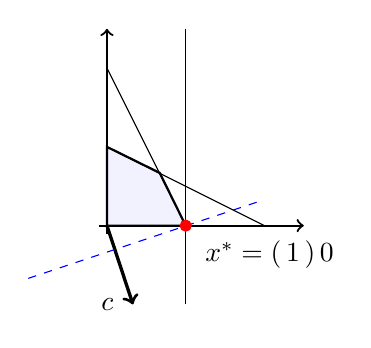
\begin{tikzpicture}[scale=1]
\draw[color=black, thick, ->] (0,-0.1)--(0,2.5);
\draw[color=black, thick, ->] (-0.1,0)--(2.5,0);
\draw[color=black, fill=blue!5, thick] (0,0)--(0,1)--(0.67,0.67)--(1,0)--(0,0);
\draw[color=black] (0,2)--(1,0);
\draw[color=black] (0,1)--(2,0);
\draw[color=black] (1,-1)--(1,2.5);
\draw[color=black,very thick,->] (0,0)--(0.33,-1);
\draw[color=blue,dashed] (-1,-0.67)--(2,0.33);
\filldraw[red] (1,0) circle (2pt);
\node (A1) at (1,0)  [label=-30:{$\vct{x}^*=\begin{pmatrix}1\\0\end{pmatrix}$}] {};
\node (A2) at (0.33,-1)  [label=180:{$c$}] {};
\end{tikzpicture}

As anchor point $\vct{p}$ we can just choose a multiple $c\vct{w}$ that is on the plane, i.e., that satisfies $\ip{\vct{w}}{c\vct{w}}+b=0$. This implies that $c=-b/\norm{\vct{w}}^2$, and consequently $\vct{p} = -(b/\norm{\vct{w}}^2 \vct{w}$. The distance is then
\begin{equation*}
  d_+ = \ip{\vct{x}+\frac{b}{\norm{\vct{w}}^2}\vct{w}}{\frac{\vct{w}}{\norm{\vct{w}}}} = \frac{1}{\norm{\vct{w}}}.
\end{equation*}
Similarly, we get $d_-=1/\norm{\vct{w}}$. The margin of this particular separating hyperplane is thus $d=2/\norm{\vct{w}}$. If we want to find a hyperplane with {\em smallest} margin, we thus have to solve the quadratic optimization problem

\begin{align*}
\minimize & \frac{1}{2}\norm{\vct{w}}^2\\
\subjto & y_i(\vct{w}^{\trans}\vct{x}_i+b)-1 \geq 0, \quad 1\leq i\leq n.
\end{align*}

Note that $b$ is also an unknown variable in this problem! 
The factor $1/2$ in the objective function is just to make the gradient look nicer. The Lagrangian of this problem is

\begin{align*}
\mathcal{L}(\vct{w},b,\vct{\lambda}) &= \frac{1}{2}\norm{\vct{w}}^2 - \sum_{i=1}^m \lambda_i y_i \vct{w}^{\trans}\vct{x}_i-\lambda_iy_ib+\lambda_i\\
&= \frac{1}{2}\vct{w}^{\trans}\vct{w}-\vct{\lambda}^{\trans}\mtx{X}\vct{w}-b\vct{\lambda}^{\trans}\vct{y}+\sum_{i=1}^m \lambda_i,
\end{align*}
 
where we denote by $\mtx{X}$ the matrix with the $y_i\vct{x}_i^{\trans}$ as rows. We can then write the conditions on the gradient with respect to $\vct{w}$ and $b$ of the Lagrangian as

\begin{align}\label{eq:lagrange-grad}
\begin{split}
 \nabla_{\vct{w}} \mathcal{L}(\vct{w},b,\vct{\lambda}) & = \vct{w}+\mtx{X}^{\trans}\vct{\lambda} = \zerovct \\
 \frac{\partial \mathcal{L}}{\partial b}(\vct{w},b,\vct{\lambda}) &= \vct{y}^{\trans}\vct{\lambda} = 0.
 \end{split}
\end{align}

Replacing $\vct{w}$ by $-\mtx{X}^{\trans}\vct{\lambda}$ and $\vct{\lambda}^{\trans}\vct{y}$ by $0$ in the Lagrangian function then gives the expression for the Lagrange dual $g(\vct{\lambda})$,
\begin{equation*}
  g(\vct{\lambda}) = -\frac{1}{2}\vct{\lambda}^{\trans}\mtx{X}\mtx{X}^{\trans}\vct{\lambda}-\sum_{i=1}^m \lambda_i.
\end{equation*}

Finally, changing the sign and the maximum with a minimum, we can formulate the Lagrange dual optimization problem as
\begin{equation}\label{eq:svm-dual}
\minimize \frac{1}{2}\vct{\lambda}^{\trans}\mtx{X}\mtx{X}^{\trans}\vct{\lambda}+ \vct{\lambda}^{\trans}\vct{e} \subjto \vct{\lambda}\geq \zerovct,
\end{equation}
where $\vct{e}$ is the vector of all ones. 

Note that there is one dual variable $\lambda_i$ per data point $\vct{x}_i$. We can find the optimal value by solving the dual problem~\eqref{eq:svm-dual}, but that does not give us automatically the weights $\vct{w}$ and the bias $b$. We can find the weights by $\vct{w}=-\mtx{X}^{\trans}\vct{\lambda}$. As for $b$, this is best determined from the KKT conditions of the problem. These can be written by combining the constraints of the primal problem with the conditions on the gradient of the Lagrangian~\eqref{eq:lagrange-grad}, the condition $\vct{\lambda}\geq \zerovct$, and complementary slackness as
\begin{align*}
   \mtx{X}\vct{w}+b\vct{y}-\vct{e} &= \zerovct\\
   \vct{\lambda}&\geq \zerovct\\
   \lambda_i (1-y_i(\vct{w}^{\trans}\vct{x}_i+b)) &= 0 \text{ for } 1\leq i\leq n\\
   \vct{w}+\mtx{X}^{\trans}\vct{\lambda} &= \zerovct\\
   \vct{y}^{\trans}\vct{\lambda} &= 0.
\end{align*}
To get $b$, we can choose one of the equations in which $\lambda_i\neq 0$, and then find $b$ by setting $b= y_i(1-y_i\vct{w}^{\trans}\vct{x}_i)$. With the KKT conditions written down, we can go about solving the problem of finding a maximum margin linear classifier using methods such as the barrier method.

\begin{example}
To be written.
\end{example}

\section{Extensions}
So far we looked at the particularly simple case where (a) the data falls into two classes, (b) the points can actually be well separated, and (c) they can be separated by an affine hyperplane. In reality, these three assumptions may not hold. We briefly discuss extensions of the basic model to account for the three situations just mentioned.

\subsection{Non-exact separation}

\subsection{Non-linear separation and kernels}

\subsection{Multiple classes}

% %-----------------------------------------------------------------------
% % End of chap1.tex
% %-----------------------------------------------------------------------
